
\section{Distribución uniforme}

La distribución uniforme continua modela el caso en el que una variable aleatoria toma
valores en un intervalo $[a,b]$ con la misma \emph{densidad} de probabilidad en todo punto.

\begin{definicion}[Distribución uniforme continua]
Una variable aleatoria continua $X$ tiene \emph{distribución uniforme continua} en el
intervalo $[a,b]$, con $a<b$, si su función de densidad está dada por
\begin{align}
 \label{eq:2.8.1}
 f(x) =
 \begin{cases}
  \dfrac{1}{b-a} & a \leq x \leq b, \\
  0 & \text{en otro caso.}
 \end{cases}
\end{align}
En este caso, escribimos $X \sim U(a,b)$.
\end{definicion}

Su función de distribución acumulada es
\begin{align}
 \label{eq:2.8.2}
 F(x) = P(X \leq x) =
 \begin{cases}
  0 & x < a, \\
  \dfrac{x-a}{b-a} & a \leq x \leq b, \\
  1 & x > b.
 \end{cases}
\end{align}

{Propiedades de la distribución uniforme} Si $X \sim U(a,b)$, entonces
\begin{align}
 \mu_X &= \frac{a+b}{2}, \\
 \s_X^2 &= \frac{(b-a)^2}{12}.
\end{align}

\begin{observacion}
La distribución uniforme es la base de la \emph{muestra aleatoria simple}: si
$X_1,\dots,X_n \sim U(0,1)$ son independientes, entonces $(X_1,\dots,X_n)$ es una muestra
uniforme en el hipercubo $[0,1]^n$.
\end{observacion}

\begin{ejemplo}
 \label{exmp:2.8.1}
El tiempo de espera de un autobús en una parada es uniforme en el intervalo
$[0,15]$ minutos. ¿Cuál es la probabilidad de que el autobús llegue en menos de
$5$ minutos? ¿Cuál es el tiempo de espera esperado?
\end{ejemplo}

\begin{solucion}
Como $X \sim U(0,15)$, la densidad es $f(x) = \frac{1}{15-0} = \frac{1}{15}$ para
$x \in [0,15]$.

La probabilidad de que llegue en menos de $5$ minutos es
\begin{align}
 P(X < 5) = \int_0^5 \frac{1}{15}\,dx = \frac{5}{15} = \frac{1}{3}.
\end{align}

El tiempo de espera esperado es
\begin{align}
 E(X) = \frac{a+b}{2} = \frac{0+15}{2} = 7.5 \text{ minutos}.
\end{align}
\end{solucion}

\lstinputlisting[language=Python]{../code/distribuciones-continuas-avanzadas/distUniforme.py}

\begin{figure}
 \centering
 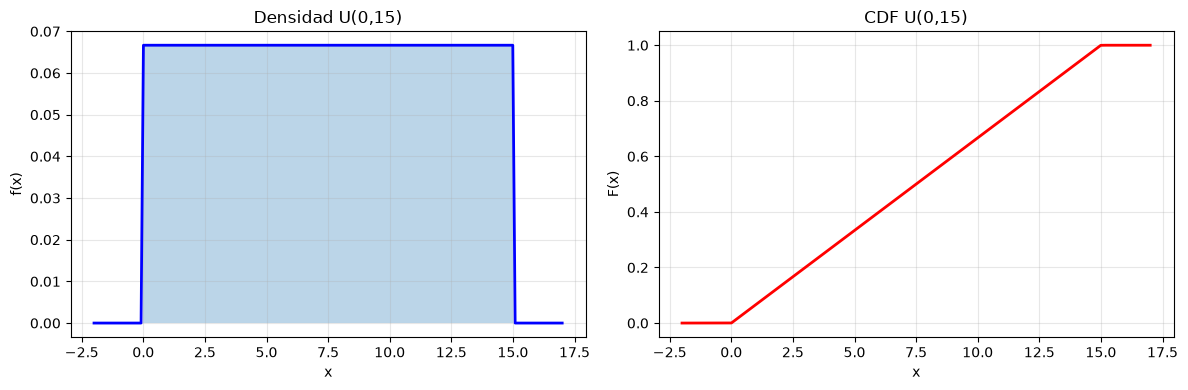
\includegraphics[height=7cm,keepaspectratio=true]{./pe/distUniforme.png}
 % distUniforme.png: 0x0 pixel, 300dpi, 0.00x0.00 cm, bb=
 \caption{Distribución uniforme continua $U(0,15)$: densidad y CDF.}
 \label{fig:2.8.1}
\end{figure}


